\section{The anatomy of the engine and how it grew}\label{sec:brain}

Anaxia is a program, so its anatomy can be counted rather than described. We read it from the package itself: every module of the package, the lines of Python it holds, and the other modules it imports, found by parsing the source.\footnote{The counts of this section are computed from the repository by the program \texttt{collect\_brain.py} in the folder of the figure sources. A line is a non-blank line of Python under \texttt{src/ebllm}, an import is an import of one module of the package by another, read with Python's \texttt{ast} module, and the history is the sequence of merges on the main branch, each read at its own commit. The numbers in the text are written into it by a second program from the same files, so that the prose and the package cannot disagree.} The package has \brainModules{} modules, \brainLines{} lines and \brainImports{} imports between modules. They fall into nine parts, and Fig.~\ref{fig:anatomy} lays them out in the order a problem passes through them, the order of the brain map of Appendix~\ref{sec:brains}: what the engine senses, what it integrates, what it does, and what it feeds back to itself.

\begin{figure*}[t]
\centering
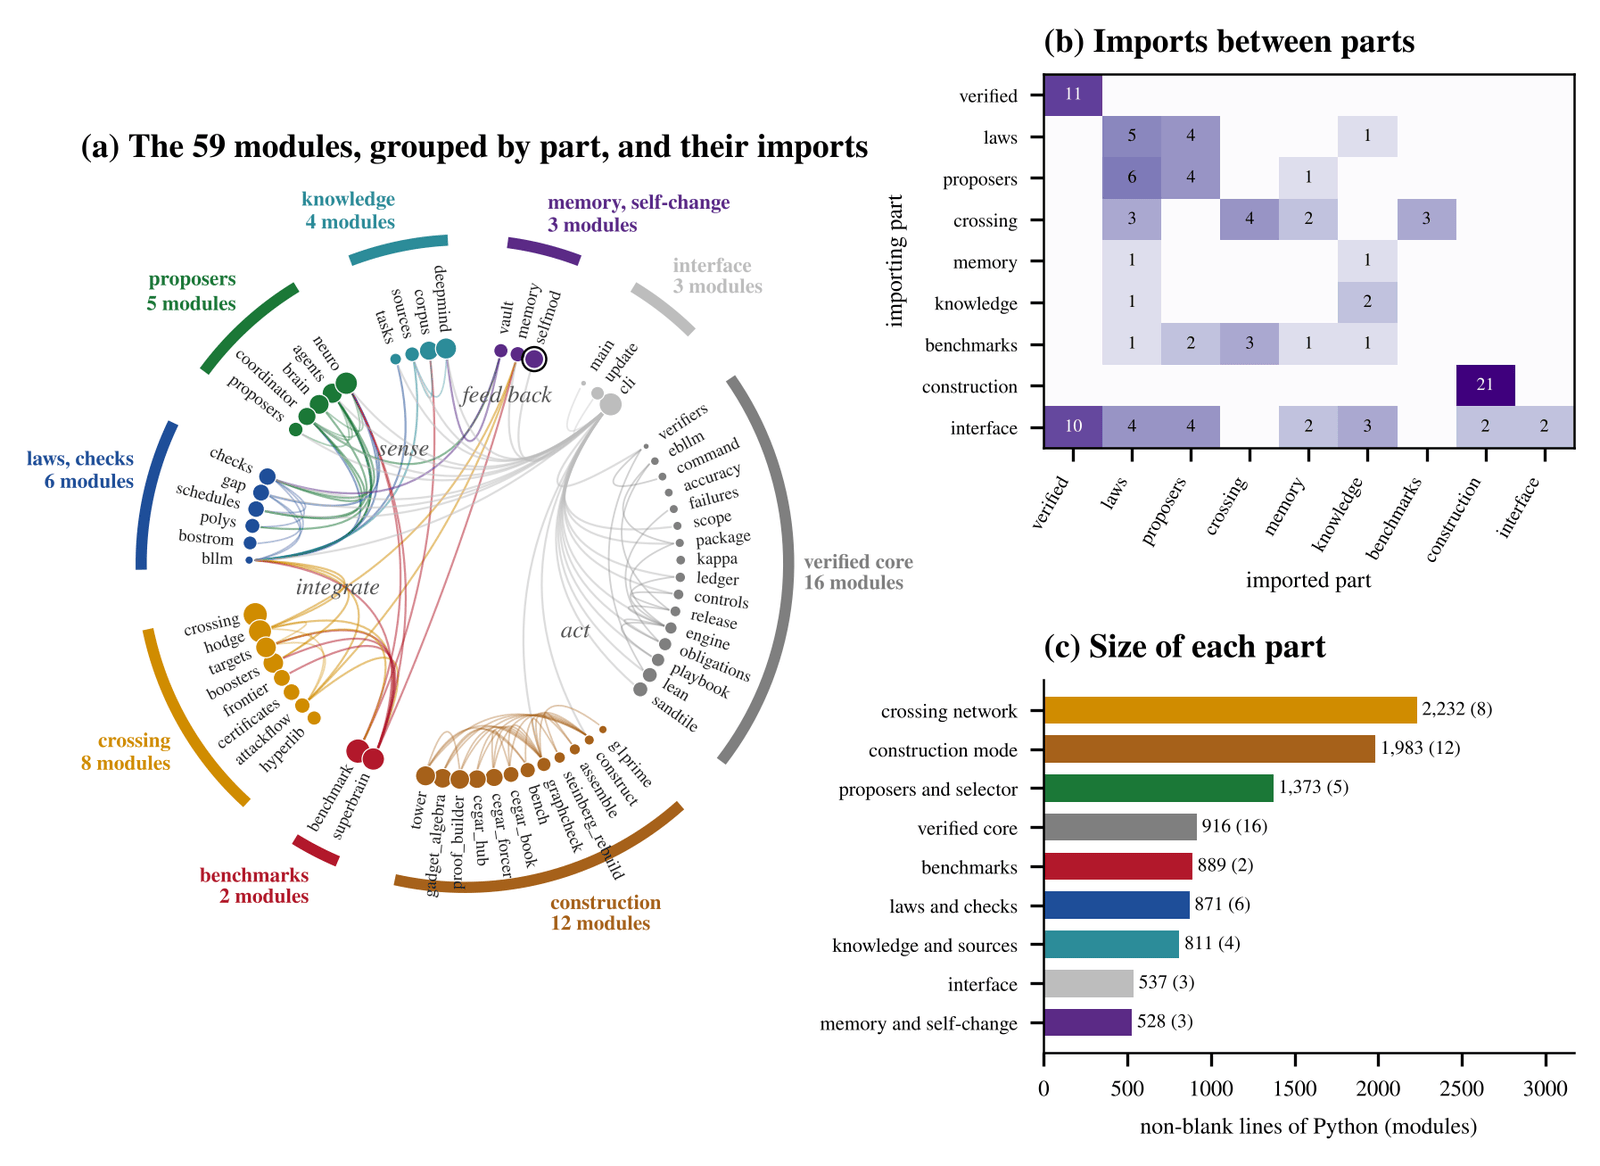
\includegraphics[width=\textwidth]{figures/fig_anatomy}
\Description{Left: the modules of the package on a circle, grouped by part, with curved lines for the imports. Upper right: a heat map of imports between parts. Lower right: horizontal bars of the lines of Python in each part.}
\caption{The anatomy of Anaxia, read from its source. (a) Each dot is a module, its area proportional to its lines of Python, coloured by part; each curve is an import, drawn inside the circle between parts and close to the rim within a part. The parts are grouped by what they do: sensing (knowledge and proposers), integrating (laws and the crossing network), acting (benchmarks, construction mode, the verified core and the interface) and feeding back (memory and the learn-from-failure loop). The four modules built last are ringed: the learn-from-failure loop and the screens in memory, and the lattice polytopes and definition repair in construction mode. (b) Imports between parts: the entry in row $i$ and column $j$ counts the imports of a module of part $j$ by a module of part $i$. (c) Lines of Python in each part, with the number of its modules in brackets.}
\label{fig:anatomy}
\end{figure*}

\subsection{Nine parts}\label{ssec:parts}

The \emph{core} is the first stage of the engine: the schedules of the entropy law, a generator interface and the checks of a verified release. It has \brainModCore{} modules and \brainLocCore{} lines, and the rest of the engine still calls it whenever a candidate must be scheduled. The \emph{laws} are the code of Sections~\ref{sec:entropy} to~\ref{sec:towers}: the checks, the entropy and R\'enyi schedules, the gap law and its estimators, in \brainModLaws{} modules and \brainLocLaws{} lines. The \emph{proposers} are the four proposers, the agents, the coordinator and the spiking selector of Proposition~\ref{prop:spiking} (\brainModProposers{} modules, \brainLocProposers{} lines). The \emph{crossing network} is the largest part, \brainModCrossing{} modules and \brainLocCrossing{} lines: typed crossing, boosters, target points, the attack channel, the Hodge agent and the certificates that the refuter reads. \emph{Memory} holds the shared store, the vault of accepted results, the learn-from-failure loop of Section~\ref{sec:selfmod} and the screens of Section~\ref{ssec:screens} (\brainModMemory{} modules, \brainLocMemory{} lines). \emph{Knowledge} holds the libraries of literature constructions, the stepwise corpora and the registry of sources (\brainModKnowledge{} modules, \brainLocKnowledge{} lines). The \emph{benchmarks} are the five problems of Section~\ref{sec:benchmark} and the comparison of whole systems (\brainModBenchmarks{} modules, \brainLocBenchmarks{} lines). \emph{Construction mode}, with the tower of builders, the lattice polytopes of the seed conjecture and definition repair, has \brainModConstruction{} modules and \brainLocConstruction{} lines. The \emph{interface} is the command \texttt{anaxia}, with \brainCommands{} subcommands, and the code that tells a running copy that a newer image exists (\brainModInterface{} modules, \brainLocInterface{} lines).

\subsection{Where the imports run}

Of the \brainImports{} imports, \brainWithin{} stay inside a part and \brainBetween{} cross from one part to another (Fig.~\ref{fig:anatomy}(b)). Two features of the wiring explain how the engine behaves. The command line imports far more modules than any other module does, because every capability of the engine is reached through it, so that it plays the part of the motor output of the brain map. In the other direction, the module imported most is \texttt{\brainHub}, imported by \brainHubIn{} modules: every object that construction mode keeps, whether it comes from the builder, from a satisfiability search, from a layer of the tower or from an assembly, passes through that one gate before it counts. That is the design of Section~\ref{ssec:construct} seen from the outside: many searches, one check that shares no code with any of them.\footnote{The gate is imported by the builder, the algebra of gadgets, the three exists-forall searches (book embedding, compressed hubs and plain forcers), the search for the first gadget, the rebuild and the assembly of Steinberg's counterexample, the tower and the command line, and by none of the modules of the crossing network, whose checks are programs of their own. A search that imported a private check of its own would show up in Fig.~\ref{fig:anatomy}(a) as a module with no curve to the gate.}

The memory sits between the sensing and the acting parts and is imported by both. The loop of Section~\ref{sec:selfmod} adds one module to it and one table to the store, and changes nothing else: an attempt that fails writes one record, and the next attempt reads the rule book that the record changed.

% generated by figures/src/make_tables_round7.py; do not edit
\begin{table*}[t]
\caption{Every release of Anaxia, read from the repository at the tagged commit of each release. Lines are non-blank lines of Python in the package; tests are test methods; Lean counts the theorems of the paper and of the engine. Times are UTC. The DOI column gives the record number of the version DOI \texttt{10.5281/zenodo.}$N$.}
\label{tab:releases}
\centering
\footnotesize
\setlength{\tabcolsep}{3.5pt}
\begin{tabular}{@{}p{0.058\textwidth}p{0.085\textwidth}p{0.062\textwidth}p{0.055\textwidth}p{0.04\textwidth}p{0.055\textwidth}p{0.427\textwidth}p{0.07\textwidth}@{}}
\toprule
\rr Release & \rr Merged & \rr Modules & \rr Lines & \rr Tests & \rr Lean & \rr What it added & \rr DOI \\
\midrule
\rr 1.0.0 & \rr 10 Oct, 18:21 & \rr 18 & \rr 1{,}041 & \rr 26 & \rr 0/26 & \rr the verified-release core: schedules of the entropy law, checks, a generator interface & \rr \href{https://doi.org/10.5281/zenodo.23286642}{23286642} \\
\rr 2.0.0 & \rr 18 Oct, 16:35 & \rr 42 & \rr 6{,}664 & \rr 61 & \rr 0/30 & \rr the crossing network, boosters, memory, target points, agents, the five benchmarks & \rr \href{https://doi.org/10.5281/zenodo.23455686}{23455686} \\
\rr 2.0.1 & \rr 18 Oct, 17:06 & \rr 42 & \rr 6{,}670 & \rr 61 & \rr 0/30 & \rr the value $f(20)=12$ of Erd\H{o}s problem 1183 & \rr \href{https://doi.org/10.5281/zenodo.23456124}{23456124} \\
\rr 2.1.0 & \rr 19 Oct, 01:53 & \rr 44 & \rr 7{,}224 & \rr 68 & \rr 59/38 & \rr the Hodge agent, the container image, the command \texttt{anaxia}, this paper and its Lean development & \rr \href{https://doi.org/10.5281/zenodo.23462639}{23462639} \\
\rr 3.0.0 & \rr 19 Oct, 04:39 & \rr 58 & \rr 9{,}837 & \rr 102 & \rr 65/38 & \rr construction mode, the DeepMind intake, the tower $B^{n}$ of builders, the registry of sources & \rr \href{https://doi.org/10.5281/zenodo.23464390}{23464390} \\
\rr 3.0.1 & \rr 19 Oct, 04:46 & \rr 58 & \rr 9{,}837 & \rr 102 & \rr 65/38 & \rr paper: the version DOI of 3.0.0 & \rr \href{https://doi.org/10.5281/zenodo.23464490}{23464490} \\
\rr 3.0.2 & \rr 19 Oct, 06:40 & \rr 58 & \rr 9{,}837 & \rr 102 & \rr 65/38 & \rr paper: compiles on TeX Live 2026; plain abstract & \rr \href{https://doi.org/10.5281/zenodo.23466863}{23466863} \\
\rr 3.0.3 & \rr 19 Oct, 06:53 & \rr 58 & \rr 9{,}837 & \rr 102 & \rr 65/38 & \rr paper: compact figures & \rr \href{https://doi.org/10.5281/zenodo.23467113}{23467113} \\
\rr 3.0.4 & \rr 19 Oct, 07:17 & \rr 58 & \rr 9{,}837 & \rr 102 & \rr 65/38 & \rr paper: layout of the appendices & \rr \href{https://doi.org/10.5281/zenodo.23467544}{23467544} \\
\rr 3.0.5 & \rr 19 Oct, 08:46 & \rr 58 & \rr 9{,}837 & \rr 102 & \rr 65/38 & \rr paper: wording of the abstract & \rr \href{https://doi.org/10.5281/zenodo.23469389}{23469389} \\
\rr 3.1.0 & \rr 19 Oct & \rr 60 & \rr 10{,}436 & \rr 131 & \rr 65/44 & \rr the learn-from-failure loop and its log; covers and descents of reflexive polytopes; the seed benchmark & \rr \anaxiaDOIshort \\
\bottomrule
\end{tabular}
\end{table*}


\subsection{How the engine grew}\label{ssec:growth}

The engine was built in five stages, each archived when it was finished (Table~\ref{tab:releases}).\footnote{A stage is an archived version whose engine differs from the one before it. Each stage is kept with its own DOI, so any of them can be rebuilt and run, and the counts of Table~\ref{tab:releases} and Fig.~\ref{fig:growth} are read from the commit archived for each stage.} The first, archived on 10 October 2026, had \brainFirstModules{} modules, \brainFirstLines{} lines and \brainFirstTests{} tests. The fifth has \brainModules{} modules, \brainLines{} lines and \brainTests{} tests, about \brainGrowth{} times as many lines, and \brainLeanPaper{} theorems of this paper and \brainLeanEngine{} of the engine proved in Lean. Fig.~\ref{fig:growth} shows the growth part by part and merge by merge.

\begin{figure*}[t]
\centering
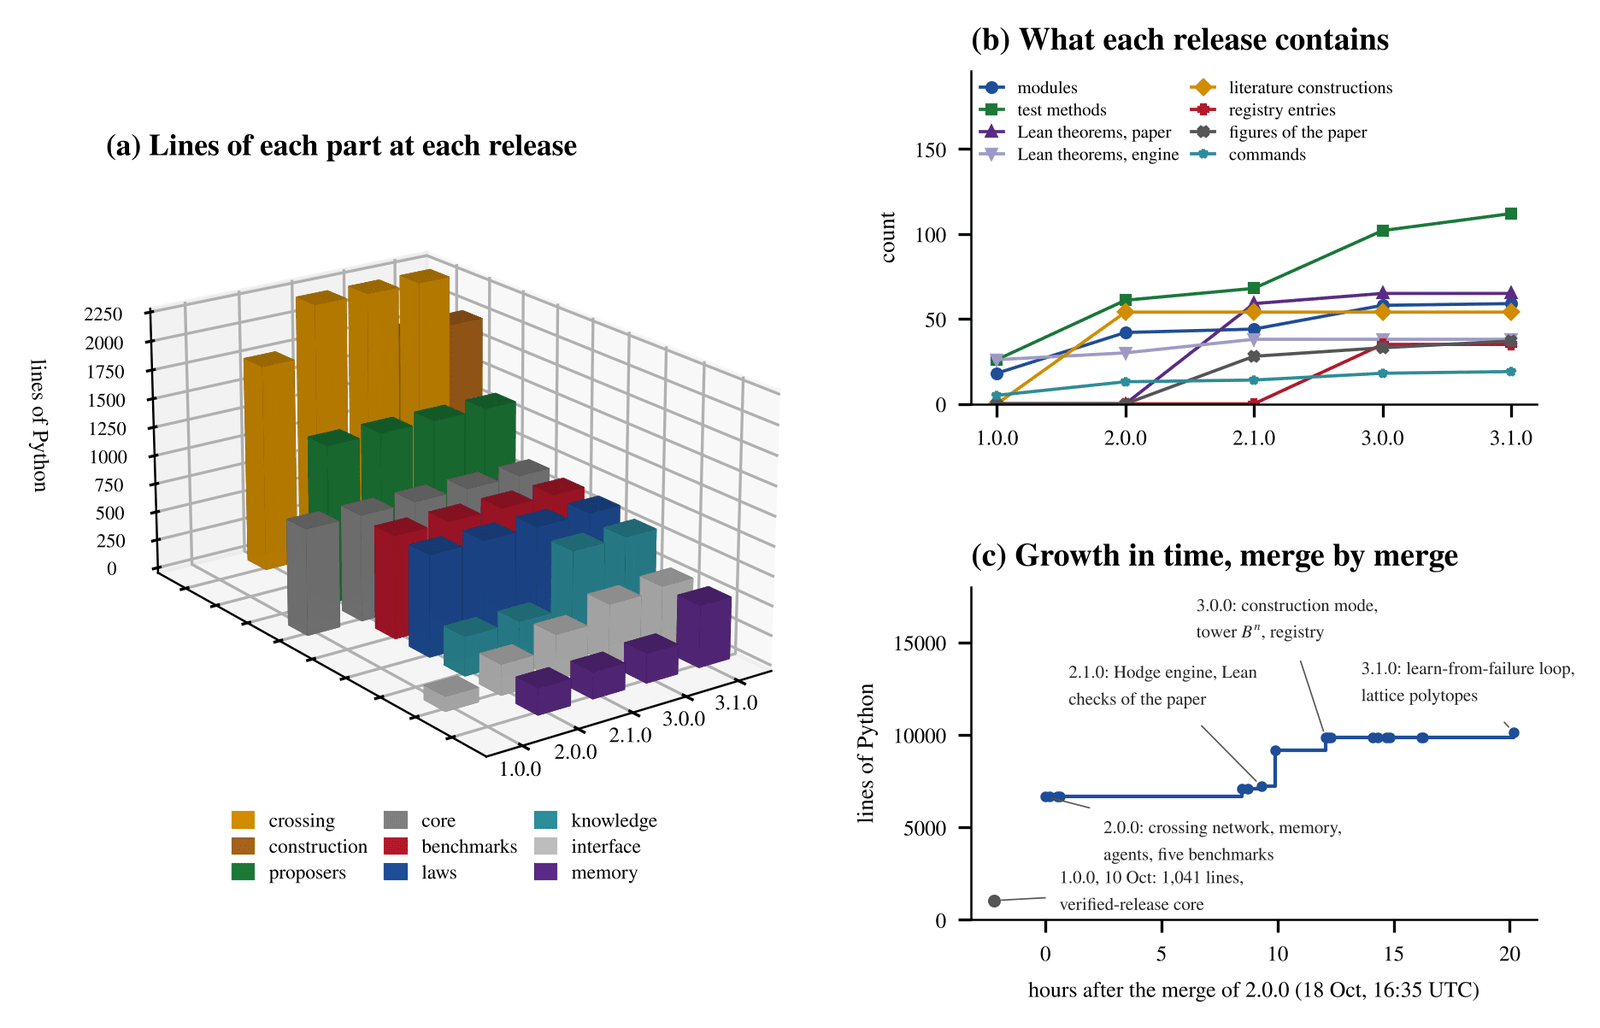
\includegraphics[width=\textwidth]{figures/fig_growth}
\Description{Left: three-dimensional bars of the lines of Python of each part at five stages. Upper right: line plot of counts of modules, tests, Lean theorems, library entries, registry entries, figures and commands per stage. Lower right: step plot of total lines against hours.}
\caption{How Anaxia grew. (a) Lines of Python in each part at each of the five stages; the parts are ordered by size at the last stage, the smallest in front, and a part absent from a stage has no bar. (b) What each stage contains: modules, test methods, Lean theorems of the paper and of the engine, literature constructions in the libraries, entries of the registry of sources, figures of the paper and subcommands of \texttt{anaxia}. (c) The total number of lines after every merge on the main branch, against the hours since the merge of stage~II; stage~I, nine days earlier, is drawn at the left.}
\label{fig:growth}
\end{figure*}

Three things stand out. First, the growth came in steps, each a new kind of part rather than more of an old one: the second stage brought the crossing network, memory, the agents and the benchmarks together and multiplied the size of the engine by six; the third, the Hodge agent and the Lean development of this paper; the fourth, construction mode and the tower; and the fifth, the loop that changes the engine's own rules, the screens it learned from failures, and the lattice polytopes on which it crossed the sub-benchmark of Section~\ref{sec:seed}. Second, the tests grew with the code, from \brainFirstTests{} methods to \brainTests{}, and from the third stage on every stage has carried a Lean development whose theorems depend only on the three standard axioms (Appendix~\ref{app:checks}). Third, most of the growth happened in one day: of the merges on the main branch, all but the first two fall after 16:35 UTC on 18 October.\footnote{The step plot of Fig.~\ref{fig:growth}(c) has long flat runs between the stages. They are merges that changed the paper and its checks and left the engine as it was; the engine itself grew in the five steps of the table.}

What the counts do not show is where the parts came from. Each new part was written after a run of the stage before failed in a way that its log could name. The crossing network was built because single proposers drew ill-typed pairs; construction mode, because crossing has nothing to combine where an object is missing; the tower, because a builder with one strategy stalled at the second gadget of \cite{CHK17}; and the loop of the next section, because those failures and their repairs had been written in prose. In the fifth stage they became records that the engine reads, and the screens are the rules those records left behind.
